Nel presente capitolo viene inizialmente introdotta l'entità fisica a fondamento di tutto il lavoro: la radiazione elettromegnetica;
in seguito vengono riportati i materiali da cui sono stati estratti i dati per le analisi e gli strumenti utilizzati nelle elaborazioni.


\section{La radiazione elettromagnetica}
Gli strumenti di acquisizione di immagini aeree e satellitari sono sensibili a determinate lunghezze d'onda della radiazione elettromagnetica (\cref{graph:el-mag-radiation}), cioè sono in grado di registrarne solo alcune porzioni (bande).
L'occhio umano può distinguere solo le bande del visibile, mentre i sensori artificiali possono acquisire altre bande della radiazione.
%
\begin{figure}
	\centering
	\tikzsetnextfilename{electromagnetic_radiation}
\begin{tikzpicture}[fill between/on layer={axis grid}]
	\begin{axis}[
		xlabel={Lunghezza d'onda},
		xticklabel style = {font=\tiny,yshift=0.2ex},
		xmin=10^-5,
		xmax=10^9,
		x unit=\si{\micro\meter},
		xmode=log,
		ymin=0,
		ymax=1,
		height=3cm,
		width=\textwidth,%12.2cm,
		yticklabels={},
		ytick=\empty,
		legend cell align=left,
		legend style={
			at={(0.5,-0.8)},%(0.85,-0.77)},
			anchor=north,
			legend columns=4,
			}
	]
	\addplot[draw=none, name path=start, forget plot] coordinates{(10^-5,0)(10^-5,1)};
	\addplot[draw=none, name path=gamma, forget plot] coordinates{(10^-3,0)(10^-3,1)};
	\addplot[draw=none, name path=xrays, forget plot] coordinates{(10^-2,0)(10^-2,1)};
	\addplot[draw=none, name path=uv, forget plot] coordinates{(0.4,0)(0.4,1)};
	\addplot[draw=none, name path=visible, forget plot] coordinates{(0.7,0)(0.7,1)};
	\addplot[draw=none, name path=ir, forget plot] coordinates{(10^2.5,0)(10^2.5,1)};
	\addplot[draw=none, name path=microwave, forget plot] coordinates{(10^5,0)(10^5,1)};
	\addplot[draw=none, name path=radiowave, forget plot] coordinates{(10^9,0)(10^9,1)};
	\addplot[violet!20, area legend] fill between[of=start and gamma];
	\addlegendentry{Raggi $\gamma$}
	\addplot[violet!60, area legend] fill between[of=gamma and xrays];
	\addlegendentry{Raggi X}
	\addplot[violet, area legend] fill between[of=xrays and uv];
	\addlegendentry{Ultravioletti}
	\addplot[shading=visiblelight, area legend] fill between[of=uv and visible];
	\addlegendentry{Luce visibile}
	\addplot[red, area legend] fill between[of=visible and ir];
	\addlegendentry{Infrarosso}
	\addplot[Bittersweet, area legend] fill between[of=ir and microwave];
	\addlegendentry{Microonde}
	\addplot[Brown, area legend] fill between[of=microwave and radiowave];
	\addlegendentry{Onde radio}
	\end{axis}
\end{tikzpicture}

	\caption[la radiazione elettromagnetica]{la radiazione elettromagnetica con le sue lunghezze d'onda.}
	\label{graph:el-mag-radiation}
\end{figure}
%
\\
Le immagini nel visibile sono solitamente suddivise nelle bande del Rosso, Verde e Blu (\emph{Red}, \emph{Green}, \emph{Blue}, R-G-B); ognuna indica la quantità di colore presente; la combinazione di queste quantità di colore restituisce l'immagine a colori.
\\
Per poter osservare immagini con bande diverse dal visibile si sostituisce una o più bande R-G-B con le bande in questione.
Ad esempio, è possibile sostituire la banda del Rosso con quella dell'Infrarosso (IR): la quantità di colore del Rosso sarà rimpiazzata dalla quantità di colore dell'Infrarosso.
Il risultato sarà un'immagine riconoscibile dall'occhio umano, ma in falsi colori (\cref{fig:confronto-bande-intro}).
%
\begin{figure}
	\centering
	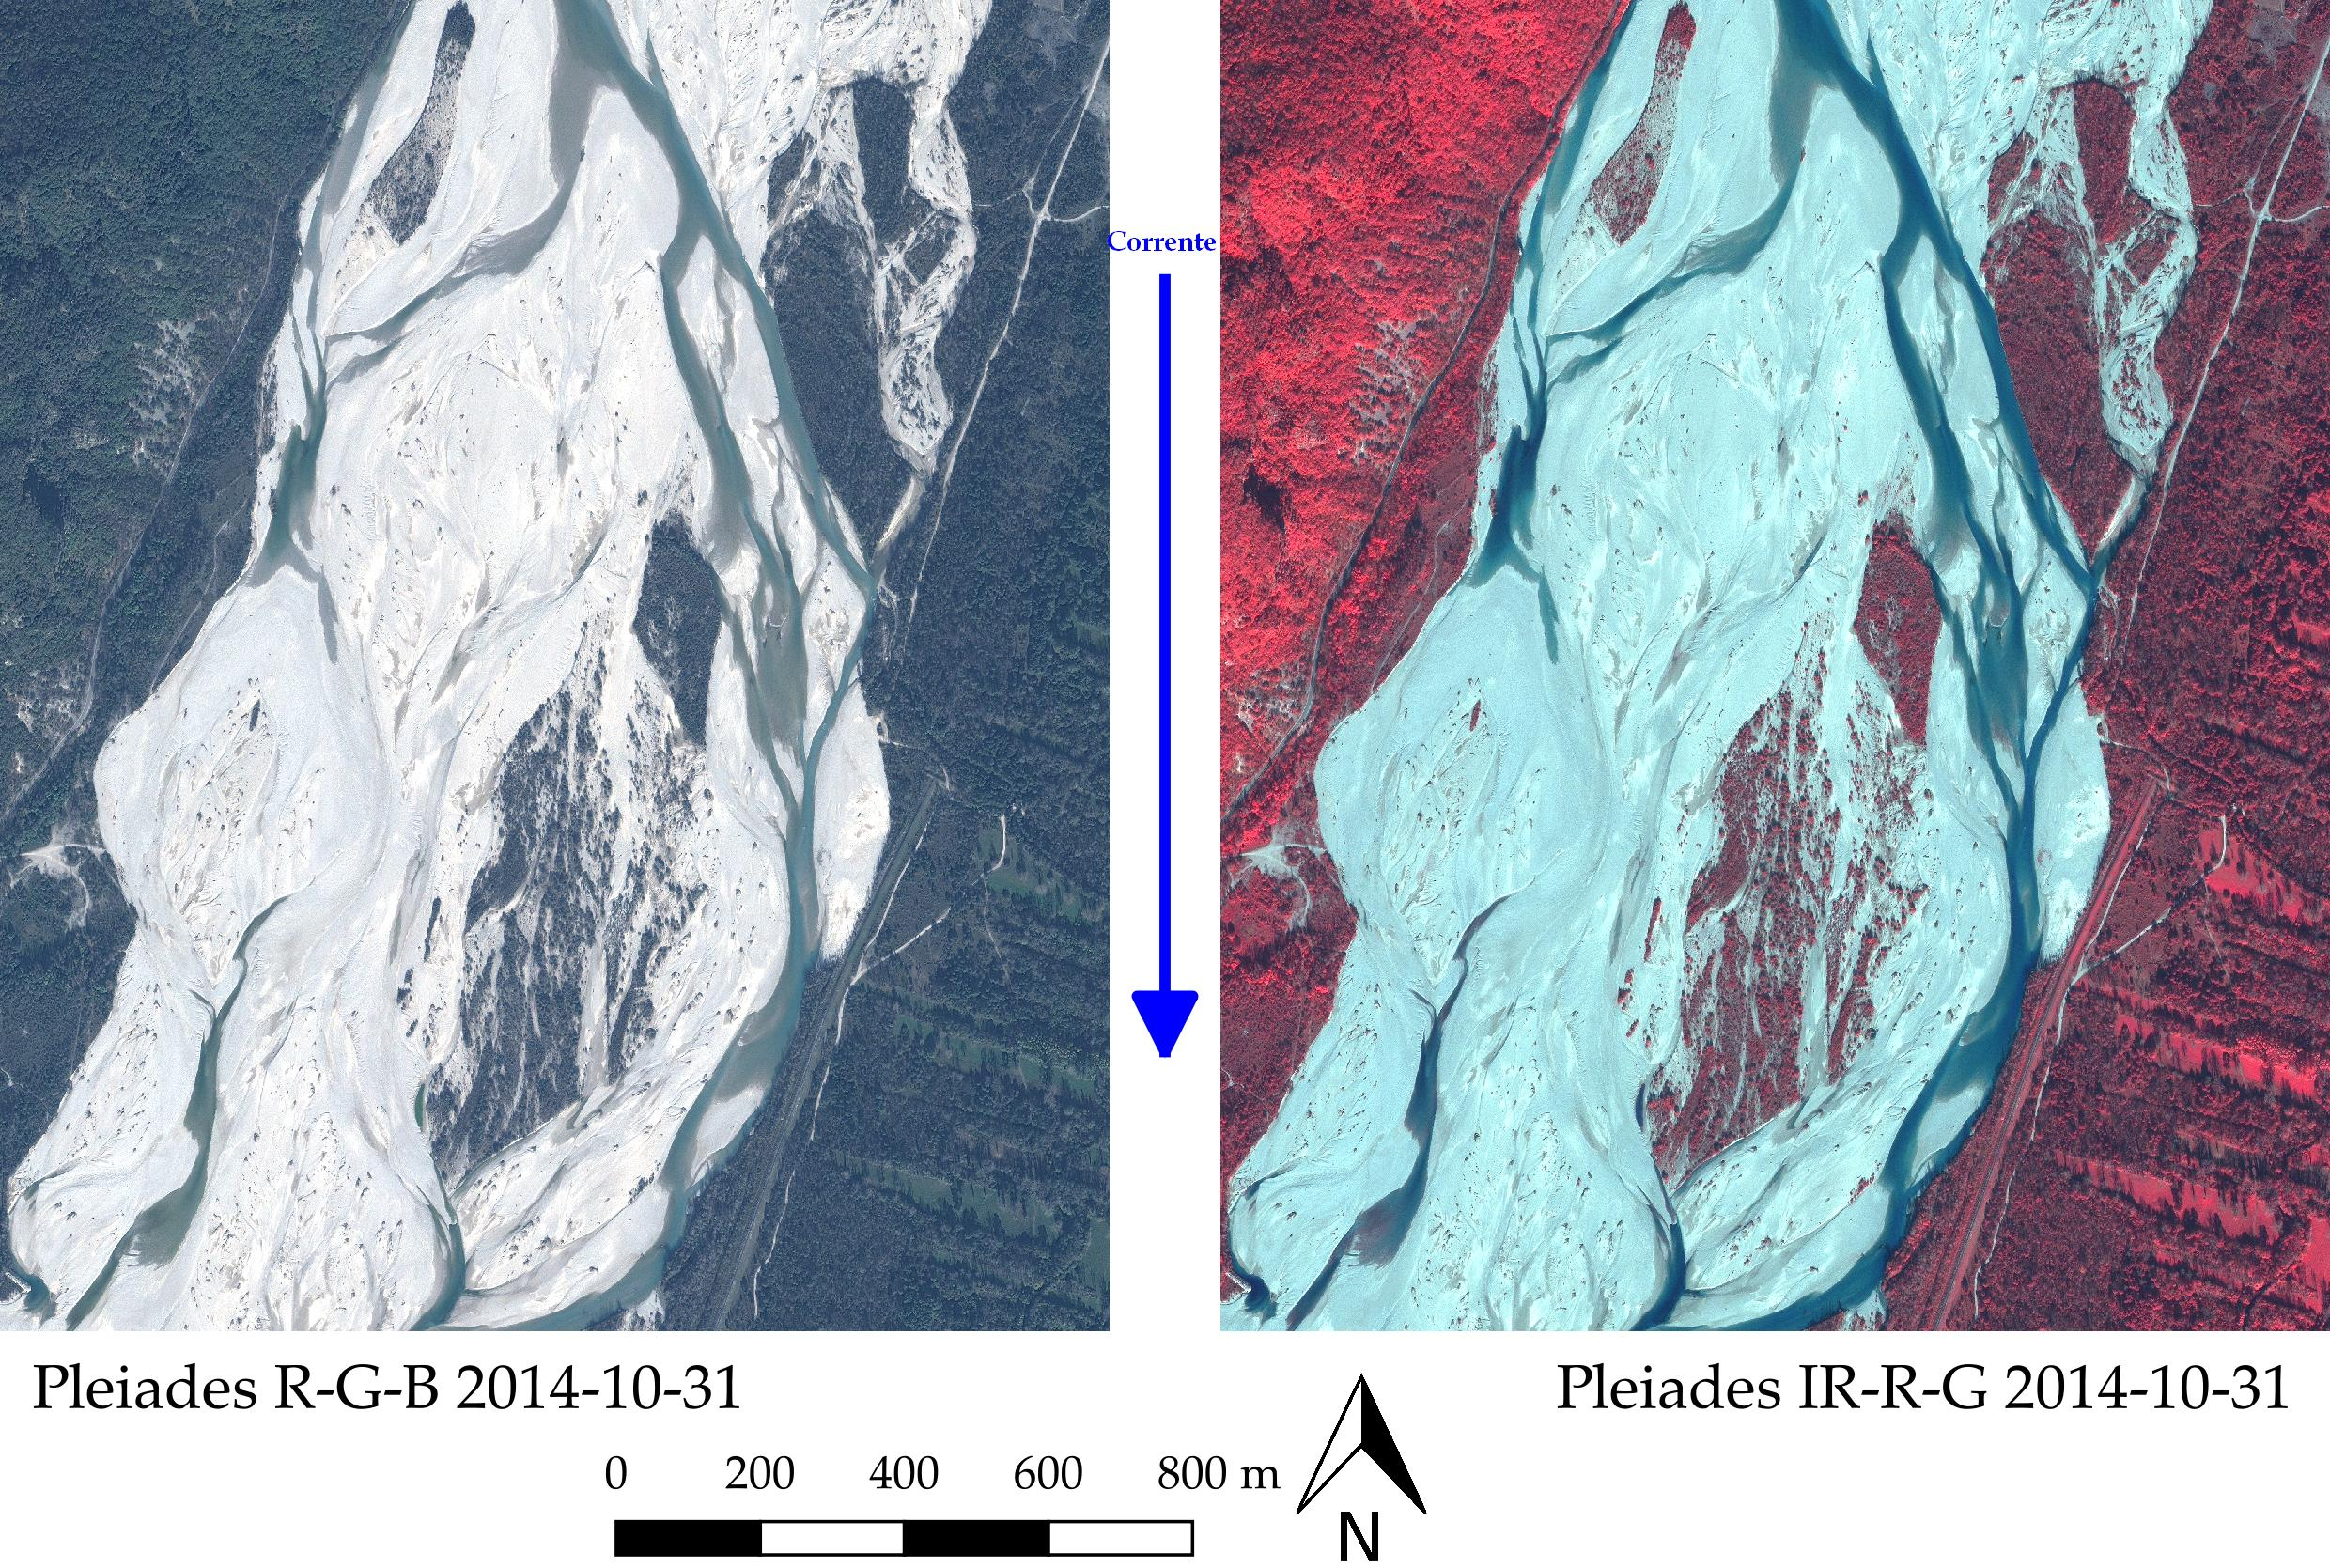
\includegraphics[width=\textwidth]{files/confronto_bande_intro.jpeg}
	\caption[confronto immagini R-G-B e IR-R-G]{confronto di un'immagine in veri colori (R-G-B, a sinistra) con una in falsi colori (IR-R-G, a destra); quest'ultima evidenza la presenza di vegetazione viva rispetto alla ghiaia in alveo e all'acqua nei canali.}
	\label{fig:confronto-bande-intro}
\end{figure}
%
\\
Questo procedimento serve per distinguere più facilmente alcuni elementi e oggetti presenti nelle immagini; per esempio la vegetazione viva riflette particolarmente la banda dell'Infrarosso più vicina al Rosso.



\section{Materiali}
\subsection{Immagini satellitari e rilievi aerei}
Nelle immagini satellitari multibande sia acquisite che di proprietà dell'Università degli Studi di Trento sono state considerate le bande del \emph{Near-InfraRed}~(NIR) e del \emph{Red}~(R), in quanto permettono di distinguere la vegetazione dalle altre coperture del suolo;
le immagini provengono dalle seguenti missioni:
%
\begin{itemize}
	\item satellite Terra, sensore \AST{} Livello~1T (ottenuti in data~21~luglio~2018 e~30~settembre~2018 \squarecite{data:ASTER});  
		\\
		NIR (Banda~3N)~\SIrange[range-phrase={-}]{0.78}{0.86}{\micro\m};
		\\
		R (Banda~2)~\SIrange[range-phrase={-}]{0.63}{0.69}{\micro\m};
	\item costellazione \Pl{} 
	%\href{https://pleiades.cnes.fr/en/PLEIADES/index.htm}{Centre National d'Etudes Spatiales}
	(Centre National d'Etudes Spatiales\footnote{\texttt{https://pleiades.cnes.fr/en/PLEIADES/index.htm}}), immagini acquistate dall'Università degli Studi di Trento; 
		\\
		NIR~\SIrange[range-phrase={-}]{0.74}{0.94}{\micro\m};
		\\
		R~\SIrange[range-phrase={-}]{0.59}{0.71}{\micro\m};
	\item satellite \Se{}A-B, sensore~MSI Livello~1C (ottenuti in data 21~luglio 2018 e~21~novembre~2018 tramite il
	%\href{http://scihub.copernicus.eu/}{Copernicus Open Access Hub}
	Copernicus Open Access Hub\footnote{\texttt{http://scihub.copernicus.eu/}});
		\\
		NIR (Banda~8)~\SIrange[range-phrase={-}]{0.763}{0.908}{\micro\m};
		\\
		R (Banda~4)~\SIrange[range-phrase={-}]{0.645}{0.683}{\micro\m};
	\item satellite \WV{}
	%\href{satimagingcorp.s3.amazonaws.com/site/pdf/WV1\_{}WV2\_{}SpectralResponse.pdf}{DigitalGlobe}
	(DigitalGlobe\footnote{\texttt{satimagingcorp.s3.amazonaws.com/site/pdf/WV1\_{}WV2\_{}SpectralResponse.pdf}}), immagini acquistate dall'Università degli Studi di Trento;
		\\
		NIR (Banda~MS1)~\SIrange[range-phrase={-}]{0.770}{0.895}{\micro\m};
		\\
		R (Banda~MS2)~\SIrange[range-phrase={-}]{0.630}{0.690}{\micro\m}.
\end{itemize}
%
Le immagini sono state selezionate secondo i seguenti criteri:
%
\begin{itemize}
	\item minima copertura nuvolosa del tratto di studio;
	\item data compresa tra metà aprile e fine ottobre, che è il periodo vegetativo delle piante decidue (\emph{Salix spp.}, \emph{Populus nigra}) che caratterizzano le isole fluviali e la piana alluvionale;
	\item basso livello dell'acqua, per evitare che alcune isole siano sommerse e non visibili;
	\item estensione di almeno qualche decina di chilometri sul tratto di studio.
\end{itemize}
%
Tutte le immagini mostrano la radianza registrata al sensore, sono geometricamente corrette tramite modelli digitali del terreno e georeferenziate secondo la proiezione UTM~33N.

Le ortofoto dell'estate~2011 provengono dal
%\href{http://www.pcn.minambiente.it/mattm/}{Portale Cartografico Nazionale del Ministero dell'Ambiente e della tutela del territorio e del mare}
Portale Cartografico Nazionale del Ministero dell'Ambiente e della tutela del territorio e del mare\footnote{\texttt{http://www.pcn.minambiente.it/mattm/}};
le ortofoto del~2013 sono state ottenute da volo
%\href{http://www.cgrspa.com/}{CGR}
CGR\footnote{\texttt{http://www.cgrspa.com/}} su commissione; 
le ortofoto del~2017 sono state ottenute da
%\href{https://www.google.com/earth/}{Google Earth}
Google Earth\footnote{\texttt{https://www.google.com/earth/}} (Map data: Google, Digital Globe, European Space Imaging).

Nei mesi di Maggio~2005, Agosto~2010 ed Ottobre~2013 (congiuntamente all'ortofoto) è stato effettuato un rilievo aereo LiDAR, grazie al quale sono a disposizione un DEM (\emph{Digital Elevation Model}) e un CHM (\emph{Canopy Height Model}) per ogni anno: il primo consiste di una mappa con le quote del suolo; il secondo è una mappa di altezza della vegetazione.
Per questi rilievi si ringraziano rispettivamente il UK Natural Environment Research Council, Nicola Surian dell'Università di Padova (progetto CARIPARO) e Yasuhiro Takemon dell'Università di Kyoto.

Il DEM del~2009 proviene dal
%\href{http://irdat.regione.fvg.it/CTRN/ricerca-cartografia/}{Portale Cartografico della regione autonoma Friuli Venezia Giulia}
Portale Cartografico della regione autonoma Friuli Venezia Giulia\footnote{\texttt{http://irdat.regione.fvg.it/CTRN/ricerca-cartografia/}}.

È bene evidenziare che le mappe non hanno tutte la medesima estensione e una piccola parte non comprende tutto il tratto oggetto di studio.
Ciò limita minimamente le analisi che è possibile fare.
\\
Avendo a disposizione 25 immagini per un periodo di studio di quasi \SI{19}{\anni},  si ritiene che la risoluzione temporale sia sufficiente per interpretare i processi che hanno luogo nel Tagliamento: la distanza temporale media tra le mappe è di \SI{274}{\giorni} (circa \SI{0.75}{\anni}), quella minima di \SI{25}{\giorni} e quella massima di \SI{480}{\giorni}.
\\
La risoluzione spaziale varia da~\SIrange[range-phrase={ a }]{15}{0.5}{\m}, adeguata per poter distinguere correttamente le caratteristiche del fiume (limite dell'alveo attivo, isole, canali nella \emph{floodplain}, canali attivi, \ldots).
\\
La \cref{tab:date-orto-sat} mostra le date, la dimensione delle celle delle immagini utilizzate nell'analisi e i tratti validi per ogni immagine.
%%%
\begin{table}[p]
	\centering
	\begin{tabular}{c c S[table-format=2.2] S[range-phrase={$\div$}, list-separator={, }, list-final-separator={, }]}
		\toprule
		\textbf{Data di}		&	\textbf{Tipo}		&	{\textbf{Dimensione}}	&	{\textbf{Tratti validi}}	\\
		\textbf{acquisizione}		&	\textbf{immagine}		&	{\textbf{celle \si{[\m]}}}	&	{}	\\
		\midrule	
		2000-09-17		&	\AST{}		&	15	&	\numrange{1}{21}	\\
		2001-06-07		&	\AST{}		&	15	&	\multicolumn{1}{c}{\numrange[range-phrase={$\div$}]{3}{8}, \numrange[range-phrase={$\div$}]{21}{23}}	\\
		2002-05-18		&	\AST{}		&	15	&	\multicolumn{1}{c}{\numrange[range-phrase={$\div$}]{1}{2}, \numrange[range-phrase={$\div$}]{6}{14}}	\\
		2002-06-12		&	\AST{}		&	15	&	\numrange{14}{23}	\\
		2003-06-22		&	\AST{}		&	15	&	\multicolumn{1}{c}{\numrange[range-phrase={$\div$}]{1}{10}, \numrange[range-phrase={$\div$}]{13}{23}}	\\
		2004-10-14		&	\AST{}		&	15	&	\numrange{2}{23}	\\
		2005-05			&	Rilievo LiDAR	&	2	&	\numrange{6}{14}	\\
		2005-08-30		&	\AST{}		&	15	&	\numrange{1}{23}	\\
		2006-07-16		&	\AST{}		&	15	&	\multicolumn{1}{c}{\numrange[range-phrase={$\div$}]{1}{20}, \numrange[range-phrase={$\div$}]{22}{23}}	\\
		2007-09-21		&	\AST{}		&	15	&	\numrange{1}{23}	\\
		2008-07-05		&	\AST{}		&	15	&	\numrange{1}{23}	\\
		2009			&	DEM			&	20	&	\numrange{1}{23}	\\
		2009-07-08		&	\AST{}		&	15	&	\numrange{3}{23}	\\
		2010-08			&	Rilievo LiDAR	&	1	&	\numlist{7;8;11}	\\
		2010-09-29		&	\AST{}		&	15	&	\numrange{1}{23}	\\
		2011-06-26/07-02	&	Ortofoto	&	1	&	\numrange{6}{12}	\\
		2011-10-02		&	\AST{}		&	15	&	\numrange{1}{23}	\\
		2012-08-01		&	\AST{}		&	15	&	\numrange{1}{23}	\\
		2013-09-05		&	\AST{}		&	15	&	\numrange{1}{23}	\\
		2013-10-22		&	Ortofoto	&	0.2	&	\numlist{7;8;11;12}	\\
		2013-10-22		&	Rilievo LiDAR	&	1	&	\numlist{7;8;11;12}	\\
		2014-09-08		&	\AST{}		&	15	&	\numrange{1}{23}	\\
		2014-10-31		&	\Pl{}	&	0.5	&	\numrange{6}{14}	\\
		2015-08-13		&	\Pl{}	&	0.5	&	\numrange{6}{14}	\\
		2015-09-12		&	\Se{}	&	10	&	\numrange{1}{23}	\\
		2015-10-22		&	\Se{}	&	10	&	\numrange{1}{23}	\\
		2016-09-13		&	\Se{}	&	10	&	\numrange{1}{23}	\\
		2017-04-21		&	\Se{}	&	10	&	\numrange{1}{23}	\\
		2017-06-13		&	\Se{}	&	10	&	\numrange{1}{23}	\\
		2017-06-26/08-02	&	G-Earth	&	0.45	&	\numrange{6}{15}	\\
		2018-06-15		&	\WV{}	&	0.5	&	\numrange{7}{14}	\\
		2018-09-16		&	\Se{}	&	10	&	\numrange{1}{23}	\\
		\bottomrule
	\end{tabular}
	\caption[dettagli delle immagini e rilievi aerei utilizzati]{data e dimensione delle celle delle immagini satellitari, delle ortofoto, del DEM e dei rilievi aerei LiDAR utilizzati.}
	\label{tab:date-orto-sat}
\end{table}


\subsection{Dati idrometrici}
I dati idrometrici orari o semi-orari dal 2000-01-01 al 2018-12-21 presso l'idrometro di Villuzza~(UD) (\SI{46.181}{\degree}N, \SI{12.958}{\degree}E, quota~\SI{240}{\m} sopra il livello del medio mare, corrispondente al ponte di Pinzano) sono stati forniti dalla
%\href{http://www.protezionecivile.fvg.it/it/rete-idrometeorologica}{rete idrometeorologica della Protezione Civile della Regione Autonoma Friuli Venezia Giulia}
rete idrometeorologica della Protezione Civile della Regione Autonoma Friuli Venezia Giulia\footnote{\texttt{http://www.protezionecivile.fvg.it/it/rete-idrometeorologica}}.
Questi dati riportano l'altezza del pelo libero dell'acqua rispetto ad un livello di riferimento locale dell'idrometro.
La dinamica della morfologia del fondo del fiume non permette di ottenere una scala di deflusso (delle portate) generalmente valida; ciò comunque non costituisce un limite poiché questi dati forniscono adeguate e sufficienti informazioni sulle piene di intensità medio-elevata.
Il grafico in \cref{graph:livelli-matrix} mostra i livelli idrometrici mediati giornalmente; da questi si vede bene come le piene siano generalmente imprevedibili, come abbiano luogo generalmente nei periodi primaverili e autunnali e come si possano alternare anni caratterizzati da pochi eventi con anni che presentano molte piene importanti; si rammenta come proprio questa naturale variabilità del regime delle piene regoli l'abbondanza e la distribuzione delle specie che vivono in ambiente ripario \squarecite{Poff:1997}.
%
\begin{figure}
	\centering
	\tikzsetnextfilename{livelli_matrix}
\begin{tikzpicture}
	\begin{axis}[
		width = \textwidth,
		height = \textwidth,
		enlargelimits = 0,
		ytick distance = 1,
		xtick = {1,31,59,90,120,151,181,212,243,273,304,334,365},
		xticklabels = {{Gennaio}, {Febbraio}, {Marzo},  {Aprile}, {Maggio}, {Giugno}, {Luglio}, {Agosto}, {Settembre}, {Ottobre}, {Novembre}, {Dicembre}},
		xticklabel style = {
			rotate = 90,
		},		
		x tick label as interval,		
		colormap/jet,
		colorbar horizontal,
		colorbar style = {
			xlabel = {Media giornaliera del livello idrometrico},
			x unit = m,
		},	
		]
		\addplot[
			matrix plot*,
			mesh/cols = 365,
			shader = flat corner,
			] % ai dati è stato eliminato il 29 febbraio...! Qualcuno se ne accorgerà mai...?
        	table [x = data, y = anno, point meta = \thisrow{media-gg}] {graphics/data/Dati_Villuzza_matrix.csv};
    \end{axis}
\end{tikzpicture}
	\caption[livelli idrometrici medi giornalieri]{livelli idrometrici medi giornalieri; risulta evidente l'imprevedibilità degli eventi di piena, sebbene questi siano concentrati durante la primavera e l'autunno.}
	\label{graph:livelli-matrix}
\end{figure}

I grafici in \cref{graph:livelli-orto-sat} mostrano rispettivamente i livelli idrometrici e le date di cui si dispongono ortofoto e immagini satellitari (\AST{}, \Pl{}, \Se{}, Google~Earth, \WV{}). 
Nel secondo grafico sono riportati solamente i livelli maggiori di~\SI{1.5}{\m} per mostrare sia le piene di media intensità che quelle più elevate.
Dalla soglia di \SI{2}{\m} si assiste ad una completa connessione di pozze, canali e sorgenti tramite l'inondazione delle barre in ghiaia più alte, iniziando quindi ad esercitare effetti di disturbo sulla vegetazione \squarecite{Bertoldi:2009-2m}.
%
\begin{figure}
	\centering
	\begin{tikzpicture}
	%\begin{groupplot}
	\begin{axis}[
		%name = orto-sat,
		axis y line* = right,
		axis x line* = top,
		%height = .3\textwidth,
		width = \textwidth,
		date coordinates in = x,
		%symbolic y coords = {ASTER,PLEIADES,SENTINEL2,G-EARTH},
		xticklabel = {\year-\month-\day},
		xtick = data,
		ytick = data,
		xticklabel style = {
			rotate = 90,
			anchor = near xticklabel
		},
		enlarge x limits = 0.05,
		enlarge y limits = 0.01,
		ylabel = {Fonte},
		ymax = 3.6,
		ymin = -0.1,
		grid = none,
		only marks,
		]
		\addplot table [x=data, y=numero] {graphics/data/data-orto-sat.txt};
	\end{axis}
	%
	\begin{axis}[
		%name = stages,
		%at = {($(orto-sat.south)-(0,2cm)$)},
		%anchor = north,
		axis y line* = left,
		width = \textwidth,
		date coordinates in = x,
		xticklabel = {\year-\month-\day},
		xticklabel style = {
			rotate = 45,
			anchor = near xticklabel
		},
		enlarge x limits = 0.05,
		enlarge y limits = 0.01,
		ymax = 3.6,
		ymin = -0.1,
		ylabel = {Livello idrometrico},
		grid = major,
		no markers,
		]
		\addplot table [x=data, y=media-gg] {graphics/data/Dati_Villuzza.csv};
	\end{axis}
\end{tikzpicture}
	\tikzsetnextfilename{livelli_2m+imm}
\begin{tikzpicture}
	\begin{axis}[
		width = \textwidth,
		height = 0.5\textwidth,
		date coordinates in = x,
		date ZERO = 2000-01-01,
		xticklabel = {$\year$},
		xticklabel style = {
			rotate = 80,
			anchor = near xticklabel
		},
		xtick distance = 732,
		enlarge x limits = 0.05,
		enlarge y limits = 0.01,
		ymax = 3.7,
		ymin = 1.95,
		ylabel = {Livello idrometrico \si{[\m]}},
		grid = major,
		]
		\addplot+ 
			[red, mark=x, semithick, style=solid, mark=x]
			coordinates {(2000-09-17, 2)(2000-09-17, 3.7)};
		\addplot+ 
			[red, semithick, style=solid, mark=x]
			coordinates {(2001-06-07, 2)(2001-06-07, 3.7)};
		\addplot+
        	[red, semithick, style=solid, mark=x]
        	coordinates {(2002-05-18, 2)(2002-05-18, 3.7)};
		\addplot+
        	[red, semithick, style=solid, mark=x]
        	coordinates {(2002-06-12, 2)(2002-06-12, 3.7)};
		\addplot+
        	[red, semithick, style=solid, mark=x]
        	coordinates {(2003-06-22, 2)(2003-06-22, 3.7)};
		\addplot+
        	[red, semithick, style=solid, mark=x]
        	coordinates {(2004-10-14, 2)(2004-10-14, 3.7)};
		\addplot+
        	[green, semithick, style=solid, mark=x]
        	coordinates {(2005-05-01, 2)(2005-05-01, 3.7)};
		\addplot+
        	[red, semithick, style=solid, mark=x]
        	coordinates {(2005-08-30, 2)(2005-08-30, 3.7)};
		\addplot+
        	[red, semithick, style=solid, mark=x]
        	coordinates {(2006-07-16, 2)(2006-07-16, 3.7)};
		\addplot+
        	[red, semithick, style=solid, mark=x]
        	coordinates {(2007-09-21, 2)(2007-09-21, 3.7)};
		\addplot+
        	[red, semithick, style=solid, mark=x]
        	coordinates {(2008-07-05, 2)(2008-07-05, 3.7)};
		\addplot+
        	[red, semithick, style=solid, mark=x]
        	coordinates {(2009-07-08, 2)(2009-07-08, 3.7)};
		\addplot+
        	[green, semithick, style=solid, mark=x]
        	coordinates {(2010-08-01, 2)(2010-08-01, 3.7)};
		\addplot+
        	[red, semithick, style=solid, mark=x]
        	coordinates {(2010-09-29, 2)(2010-09-29, 3.7)};
		\addplot+
        	[green, semithick, style=solid, mark=x]
        	coordinates {(2011-07-01, 2)(2011-07-01, 3.7)};
		\addplot+
        	[red, semithick, style=solid, mark=x]
        	coordinates {(2012-08-01, 2)(2012-08-01, 3.7)};
		\addplot+
        	[red, semithick, style=solid, mark=x]
        	coordinates {(2013-09-05, 2)(2013-09-05, 3.7)};
		\addplot+
        	[green, semithick, style=solid, mark=x]
        	coordinates {(2013-10-22, 2)(2013-10-22, 3.7)};
		\addplot+
        	[red, semithick, style=solid, mark=x]
        	coordinates {(2014-09-08, 2)(2014-09-08, 3.7)};
		\addplot+
        	[black, semithick, style=solid, mark=x]
        	coordinates {(2014-10-31, 2)(2014-10-31, 3.7)};
       	\addplot+
        	[black, semithick, style=solid, mark=x]
        	coordinates {(2015-08-13, 2)(2015-08-13, 3.7)};
		\addplot+
        	[cyan, semithick, style=solid, mark=x]
        	coordinates {(2015-09-12, 2)(2015-09-12, 3.7)};
		\addplot+
        	[cyan, semithick, style=solid, mark=x]
        	coordinates {(2015-10-22, 2)(2015-10-22, 3.7)};
		\addplot+
        	[cyan, semithick, style=solid, mark=x]
        	coordinates {(2016-09-13, 2)(2016-09-13, 3.7)};
		\addplot+
        	[cyan, semithick, style=solid, mark=x]
        	coordinates {(2017-04-21, 2)(2017-04-21, 3.7)};
		\addplot+
        	[cyan, semithick, style=solid, mark=x]
        	coordinates {(2017-06-13, 2)(2017-06-13, 3.7)};
		\addplot+
        	[green, semithick, style=solid, mark=x]
        	coordinates {(2017-07-07, 2)(2017-07-07, 3.7)};
       	\addplot+
        	[violet, semithick, style=solid, mark=x]
        	coordinates {(2018-06-15, 2)(2018-06-15, 3.7)};
		\addplot+
        	[cyan, semithick, style=solid, mark=x]
        	coordinates {(2018-09-16, 2)(2018-09-16, 3.7)};
		\addplot+
        	[blue, solid, no markers]
        	table [x=data, y=media-gg] {graphics/data/Dati_Villuzza.csv};
	\end{axis}
\end{tikzpicture}
	\caption[livelli idrometrici e foto aeree - satellitari]{in alto il livello idrometrico (in blu) presso l'idrometro di Villuzza, registrato con frequenza oraria o semi-oraria. 
	In basso un ingrandimento per i livelli medi giornalieri superiori a~\SI{1.5}{\m}, che sono indice di piene con effetti non trascurabili.
	I simboli indicano le immagini satellitari e le ortofoto considerate (\AST{} in rosso, ortofoto, rilievi aerei LiDAR e G-Earth in verde, \Pl{} in nero, \Se{} in azzurro, \WV{} in viola).}
	\label{graph:livelli-orto-sat}
\end{figure}



\section{Strumenti}
Per eseguire le analisi sulle immagini aeree e satellitari sono stati utilizzati i GIS GRASS \squarecite{soft:GRASS} e QGIS \squarecite{soft:QGIS}. 
\\
Per l'estrazione delle immagini satellitari \AST{} dagli archivi \texttt{.hdf} è stato usato SCP, plugin di QGIS \squarecite{soft:SCP}. 
\\
Per il download delle ortofoto dell'estate~2017 si è utilizzato
%\href{https://github.com/sourcepole/qgis-openlayers-plugin}{OpenLayers}
OpenLayers\footnote{\texttt{https://github.com/sourcepole/qgis-openlayers-plugin}}, plugin di QGIS.
\\
Per le analisi dei dati sono stati realizzati script in Python~2.7.5 utilizzando la libreria PyGRASS\footnote{\texttt{https://grass.osgeo.org/programming7/}} \squarecite{Zambelli:2013-pygrass} e in Python~3.7.1\footnote{\texttt{https://www.python.org}}.
